\documentclass[../master/master.tex]{subfiles}

\begin{document}

%----------------------------------------------------------------------
% LECTURE 2: Construction of the Real Numbers
% Date: January 22, 2026
%----------------------------------------------------------------------
\renewcommand{\lecturenum}{2}
\renewcommand{\lecturedate}{January 22, 2026}
\renewcommand{\lecturetopic}{Construction of the Real Numbers}

\section{Lecture \lecturenum : \lecturedate}

\begin{lecturesummary}
\textbf{Lecture Overview:} We construct the real numbers $\R$ as an ordered field with the Least Upper Bound Property (LUBP) containing $\Q$ as a subfield, using Dedekind cuts. We prove key properties of $\R$: the Archimedean property and density of $\Q$ in $\R$. Using the LUBP, we establish existence of $n$th roots of positive reals via a supremum argument. We discuss decimal/ternary representations and the Cantor set. We introduce the complex numbers $\C$ and prove $\C$ is not an ordered field. Finally, we define Euclidean spaces $\R^n$ with inner products and norms, and prove the Cauchy-Schwarz inequality.
\end{lecturesummary}

\subsection{Dedekind Cuts}

\begin{summarybox}
\textbf{Section Overview:} We define Dedekind cuts as a way to construct the real numbers from the rationals.
\end{summarybox}

\begin{definition}
A \defn{cut} $\alpha \subset \Q$ is a nonempty, proper subset such that:
\begin{enumerate}
    \item \textbf{Downward closed:} If $p \in \alpha$ and $q < p$, then $q \in \alpha$.
    \item If $\sup \alpha$ exists, then $\sup \alpha \notin \alpha$.
\end{enumerate}
\end{definition}

The set of all cuts is ordered by inclusion: $\alpha \leq \beta$ if and only if $\alpha \subseteq \beta$.

\subsection{Field Operations on Cuts}

\begin{summarybox}
\textbf{Section Overview:} We define addition and multiplication on cuts to make them into an ordered field.
\end{summarybox}

\textbf{Addition:}
\[
\alpha + \beta = \{r + s \mid r \in \alpha, s \in \beta\}
\]

\textbf{Additive identity:}
\[
0^* = \{p \in \Q \mid p < 0\}
\]

\textbf{Multiplication:} For $\alpha > 0^*$ and $\beta > 0^*$:
\[
\alpha \beta = \{p \in \Q \mid p \leq rs \text{ for some } r \in \alpha, r > 0 \text{ and } s \in \beta, s > 0\}
\]

\subsection{Least Upper Bound Property}

\begin{summarybox}
\textbf{Section Overview:} We show that the set of cuts has the LUBP.
\end{summarybox}

For a nonempty set $E$ of cuts that is bounded above:
\[
\sup E = \bigcup_{\alpha \in E} \alpha
\]

\subsection{Embedding $\Q$ into $\R$}

\begin{summarybox}
\textbf{Section Overview:} We embed the rationals into the reals as a subfield.
\end{summarybox}

For $p \in \Q$, define the cut:
\[
p^* := \{q \in \Q \mid q < p\}
\]

This embedding $p \mapsto p^*$ identifies $\Q$ as a subfield of $\R$.

\subsection{Properties of $\R$}

\begin{summarybox}
\textbf{Section Overview:} Having constructed $\R$, we now explore its key properties.
\end{summarybox}

\begin{theorem}[Archimedean Property]
For any $x, y \in \R$ with $x > 0$, there exists $n \in \N$ such that $nx > y$.
\end{theorem}

\begin{proof}
By contradiction. Suppose no such $n$ exists, i.e., $nx \leq y$ for all $n \in \N$. Then the set $A = \{nx : n \in \N\}$ is bounded above by $y$. By the LUBP, $\sup A$ exists. Let $\alpha = \sup A$. Since $x > 0$, we have $\alpha - x < \alpha$, so $\alpha - x$ is not an upper bound for $A$. Thus there exists $m \in \N$ with $mx > \alpha - x$, which gives $(m+1)x > \alpha$. But $(m+1)x \in A$, contradicting that $\alpha = \sup A$.
\end{proof}

\begin{remark}
The Archimedean property ensures there are no \defn{infinitely large} elements (every element is bounded by some natural number) and no \defn{infinitesimals} (positive elements smaller than $1/n$ for all $n$). This property is essential for proving that $\Q$ is dense in $\R$.

\textbf{Example of a non-Archimedean field:} Consider the field of rational functions $\R(x)$ with the ordering where $x$ is declared to be larger than every real number (i.e., $x > r$ for all $r \in \R$). Then $x > n$ for all $n \in \N$, so the Archimedean property fails. In this field, $1/x$ is an infinitesimal: it is positive but smaller than $1/n$ for all $n \in \N$.

\begin{center}
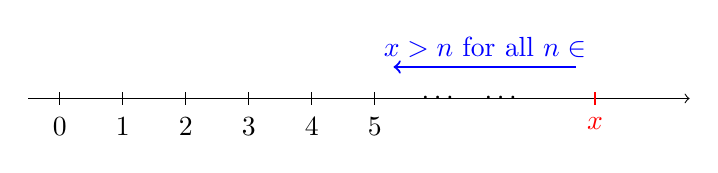
\begin{tikzpicture}[scale=0.8]
    % Draw the number line
    \draw[->] (-0.5,0) -- (10,0);

    % Draw tick marks and labels for natural numbers
    \foreach \x in {1,2,3,4,5} {
        \draw (\x,0.1) -- (\x,-0.1);
        \node[below] at (\x,-0.15) {$\x$};
    }

    % Dots to indicate continuation
    \node at (6,0) {$\cdots$};
    \node at (7,0) {$\cdots$};

    % Draw x beyond all natural numbers
    \draw[thick, red] (8.5,0.1) -- (8.5,-0.1);
    \node[below, red] at (8.5,-0.15) {$x$};

    % Arrow indicating x > n for all n
    \draw[<-, thick, blue] (5.3,0.5) -- (8.2,0.5);
    \node[above, blue] at (6.75,0.5) {$x > n$ for all $n \in \N$};

    % Label origin
    \draw (0,0.1) -- (0,-0.1);
    \node[below] at (0,-0.15) {$0$};
\end{tikzpicture}
\end{center}
\end{remark}

\begin{theorem}[Density of $\Q$ in $\R$]
For any $a, b \in \R$ with $a < b$, there exists $q \in \Q$ such that $a < q < b$.
\end{theorem}

\begin{proof}
Since $b - a > 0$, by the Archimedean property there exists $n \in \N$ such that $n(b - a) > 1$, i.e., $nb - na > 1$. Thus there exists an integer $m$ with $na < m < nb$. Then $a < \frac{m}{n} < b$, and $q = \frac{m}{n} \in \Q$.
\end{proof}

\subsection{The Roots of Reals}

\begin{summarybox}
\textbf{Section Overview:} Having constructed $\R$ with the LUBP, we can now prove that $n$th roots of positive reals exist, resolving the gap in $\Q$ where $\sqrt{2}$ was missing.
\end{summarybox}

Previously, we showed that $\sqrt{2} \notin \Q$. Now that we have constructed $\R$ with the LUBP, we can prove that $n$th roots exist.

\begin{theorem}[Existence of $n$th Roots]
For all $x \in \R_{>0}$ and for all $n \in \Z_{>0}$, there exists a unique $y \in \R_{>0}$ such that $y^n = x$.
\end{theorem}

\newpage

\begin{proof}
Let $E = \{t \in \R_{>0} : t^n < x\}$.

\textbf{$E$ is non-empty:} We have
\[
\left(\frac{x}{x+1}\right)^n < \frac{x}{x+1} < x,
\]
so $\frac{x}{x+1} \in E$.

\textbf{$E$ is bounded above:} (to be shown)

By the LUBP, $y = \sup E$ exists.

\textbf{Claim:} $y^n = x$.

\textit{Aside (Trichotomy):} Since $\R$ is a totally ordered set, for any $a, b \in \R$, exactly one of the following holds: $a < b$, $a = b$, or $a > b$. Thus for $y^n$ and $x$, exactly one of $y^n < x$, $y^n = x$, or $y^n > x$ holds. We show the first and third cases lead to contradictions.

\textbf{Case 1:} Suppose $y^n < x$. Then there exists $h > 0$ small enough such that $(y + h)^n < x$. But then $y + h \in E$, contradicting that $y = \sup E$.

\textbf{Case 2:} Suppose $y^n > x$. Then there exists $h > 0$ small enough such that $(y - h)^n > x$. But then $y - h$ is still an upper bound for $E$, contradicting that $y = \sup E$ (the \emph{least} upper bound).

Therefore $y^n = x$.
\end{proof}

\begin{notebox}
\textbf{Note to the reader:} This proof employs a fundamental technique in real analysis called a \emph{supremum argument}. The strategy is:
\begin{enumerate}
    \item \textbf{Define a set:} Construct a set $E$ of elements that are ``too small'' (i.e., $t^n < x$).
    \item \textbf{Apply LUBP:} Since $E$ is nonempty and bounded above, $\sup E$ exists---this is where we crucially use that $\R$ has the Least Upper Bound Property.
    \item \textbf{Use trichotomy:} By the trichotomy of total orders, the supremum $y$ satisfies exactly one of $y^n < x$, $y^n = x$, or $y^n > x$.
    \item \textbf{Eliminate by contradiction:} Show that $y^n < x$ contradicts $y$ being an \emph{upper} bound (we can go higher), and $y^n > x$ contradicts $y$ being the \emph{least} upper bound (we can find a smaller upper bound).
\end{enumerate}
This technique appears repeatedly throughout analysis whenever we need to prove existence of a value with a specific property. A similar technique is employed in Exercise 7 (showing the existence of the logarithm).
\end{notebox}
\newpage
\subsection{Decimals, Binaries, Ternaries}

\begin{summarybox}
\textbf{Section Overview:} We discuss representations of real numbers in different bases.
\end{summarybox}

Observe that decimal representations come in the form
\[
n_0 + \frac{n_1}{10} + \frac{n_2}{100} + \cdots = n_0 + \sum_{k=1}^{\infty} \frac{n_k}{10^k}
\]
where $n_0 \in \Z$ and $n_k \in \{0, 1, 2, \ldots, 9\}$ for $k \geq 1$.

If we consider the set of partial sums
\[
E = \left\{ n_0, \; n_0 + \frac{n_1}{10}, \; n_0 + \frac{n_1}{10} + \frac{n_2}{100}, \; \ldots \right\}
\]
then $x = \sup E$.

\begin{notebox}
\textbf{Note:} This construction is used to build the \defn{Cantor set}. Starting with the interval $[0,1]$, we iteratively remove the open middle third of each remaining interval:

\begin{center}
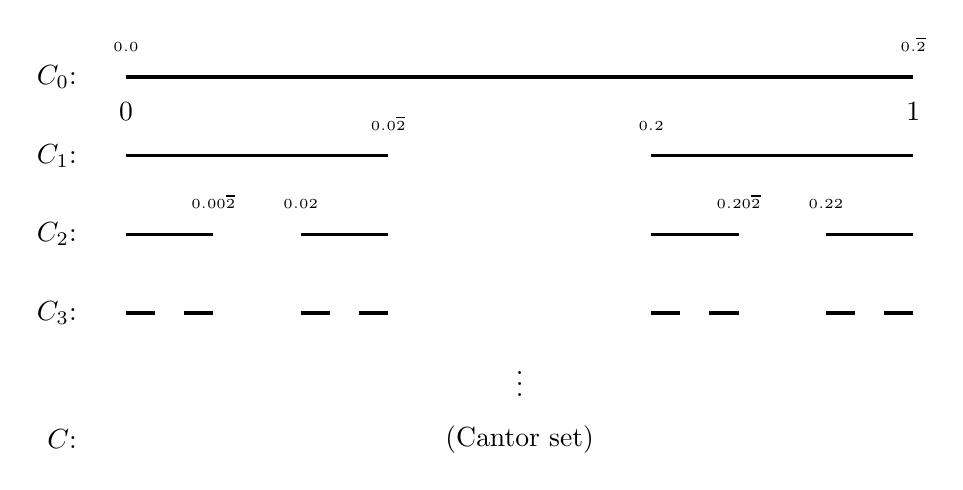
\begin{tikzpicture}[scale=10]
    % Level 0: [0,1]
    \draw[very thick] (0,0) -- (1,0);
    \node[left] at (-0.05,0) {$C_0$:};
    \node[below] at (0,-0.02) {$0$};
    \node[below] at (1,-0.02) {$1$};
    \node[above] at (0,0.02) {\tiny $0.0$};
    \node[above] at (1,0.02) {\tiny $0.\overline{2}$};

    % Level 1: [0,1/3] ∪ [2/3,1]
    \draw[very thick] (0,-0.1) -- (0.333,-0.1);
    \draw[very thick] (0.667,-0.1) -- (1,-0.1);
    \node[left] at (-0.05,-0.1) {$C_1$:};
    \node[above] at (0.333,-0.08) {\tiny $0.0\overline{2}$};
    \node[above] at (0.667,-0.08) {\tiny $0.2$};

    % Level 2: Remove middle thirds again
    \draw[very thick] (0,-0.2) -- (0.111,-0.2);
    \draw[very thick] (0.222,-0.2) -- (0.333,-0.2);
    \draw[very thick] (0.667,-0.2) -- (0.778,-0.2);
    \draw[very thick] (0.889,-0.2) -- (1,-0.2);
    \node[left] at (-0.05,-0.2) {$C_2$:};
    \node[above] at (0.111,-0.18) {\tiny $0.00\overline{2}$};
    \node[above] at (0.222,-0.18) {\tiny $0.02$};
    \node[above] at (0.778,-0.18) {\tiny $0.20\overline{2}$};
    \node[above] at (0.889,-0.18) {\tiny $0.22$};

    % Level 3
    \draw[very thick] (0,-0.3) -- (0.037,-0.3);
    \draw[very thick] (0.074,-0.3) -- (0.111,-0.3);
    \draw[very thick] (0.222,-0.3) -- (0.259,-0.3);
    \draw[very thick] (0.296,-0.3) -- (0.333,-0.3);
    \draw[very thick] (0.667,-0.3) -- (0.704,-0.3);
    \draw[very thick] (0.741,-0.3) -- (0.778,-0.3);
    \draw[very thick] (0.889,-0.3) -- (0.926,-0.3);
    \draw[very thick] (0.963,-0.3) -- (1,-0.3);
    \node[left] at (-0.05,-0.3) {$C_3$:};

    % Dots for continuation
    \node at (0.5,-0.38) {$\vdots$};
    \node[left] at (-0.05,-0.46) {$C$:};
    \node at (0.5,-0.46) {(Cantor set)};
\end{tikzpicture}
\end{center}

\noindent Here the labels are \emph{ternary} (base-3) expansions: e.g., $0.2_3 = \frac{2}{3}$, $0.02_3 = \frac{2}{9}$, $0.22_3 = \frac{8}{9}$, and $0.\overline{2}_3 = 0.222\ldots_3 = 1$.

The Cantor set $C = \bigcap_{n=0}^{\infty} C_n$ consists of all points in $[0,1]$ whose ternary (base-3) expansion contains only the digits $0$ and $2$.
\end{notebox}

\subsection{The Complex Field}

\begin{summarybox}
\textbf{Section Overview:} We introduce the complex numbers $\C$ as an extension of $\R$.
\end{summarybox}

\begin{definition}
The \defn{complex numbers} are defined as
\[
\C = \R[x] / (x^2 + 1)
\]
where each element is of the form $z = a + bi$ with $a, b \in \R$ and $i^2 = -1$.
\end{definition}

\begin{theorem}
$\C$ is not an ordered field.
\end{theorem}

\begin{proof}
By contradiction. Suppose $\C$ is an ordered field. By trichotomy, either $i > 0$ or $i < 0$ (since $i \neq 0$).

\textbf{Case 1:} If $i > 0$, then $i^2 > 0$ (since squares of nonzero elements are positive in an ordered field). But $i^2 = -1 < 0$, a contradiction.

\textbf{Case 2:} If $i < 0$, then $-i > 0$, so $(-i)^2 > 0$. But $(-i)^2 = i^2 = -1 < 0$, a contradiction.

Therefore $\C$ cannot be an ordered field.
\end{proof}

\subsection{The Euclidean Spaces}

\begin{summarybox}
\textbf{Section Overview:} We introduce Euclidean spaces $\R^n$ as spaces of ordered $n$-tuples.
\end{summarybox}

\begin{definition}
The \defn{Euclidean space} $\R^n$ is the set of all ordered $n$-tuples
\[
\vec{x} = (x_1, x_2, x_3, \ldots, x_n)
\]
where $x_i \in \R$ for each $i = 1, \ldots, n$.
\end{definition}

For $\vec{x} = (x_1, \ldots, x_n)$, $\vec{y} = (y_1, \ldots, y_n) \in \R^n$ and $c \in \R$:

\textbf{Addition:}
\[
\vec{x} + \vec{y} = (x_1 + y_1, x_2 + y_2, \ldots, x_n + y_n)
\]

\textbf{Scalar multiplication:}
\[
c\vec{x} = (cx_1, cx_2, \ldots, cx_n)
\]

\textbf{Inner product:}
\[
\langle \vec{x}, \vec{y} \rangle = \vec{x} \cdot \vec{y} = \sum_{i=1}^{n} x_i y_i = x_1 y_1 + x_2 y_2 + \cdots + x_n y_n
\]

\begin{definition}
An \defn{inner product} over $\R$ is a map $\langle \cdot, \cdot \rangle : V \times V \to \R$ that is:
\begin{itemize}
    \item Symmetric bilinear and positive definite (for real vector spaces), or
    \item Hermitian sesquilinear and positive definite (for complex vector spaces).
\end{itemize}
\end{definition}

\textbf{Properties:}
\begin{itemize}
    \item \defn{Symmetric:} $\langle x, y \rangle = \langle y, x \rangle$

    \item \defn{Hermitian:} $\langle x, y \rangle = \overline{\langle y, x \rangle}$ (conjugate symmetry)

    \item \defn{Bilinear:} Linear in both arguments:
    \begin{align*}
        \langle ax + by, z \rangle &= a\langle x, z \rangle + b\langle y, z \rangle \\
        \langle x, ay + bz \rangle &= a\langle x, y \rangle + b\langle x, z \rangle
    \end{align*}

    \item \defn{Sesquilinear:} Linear in one argument, conjugate-linear in the other:
    \begin{align*}
        \langle ax + by, z \rangle &= a\langle x, z \rangle + b\langle y, z \rangle \\
        \langle x, ay + bz \rangle &= \bar{a}\langle x, y \rangle + \bar{b}\langle x, z \rangle
    \end{align*}

    \item \defn{Positive definite:} $\langle x, x \rangle \geq 0$, with equality if and only if $x = 0$
\end{itemize}

\begin{definition}
The \defn{norm} of a vector $\vec{x}$ is defined as
\[
\|\vec{x}\| = \sqrt{\langle \vec{x}, \vec{x} \rangle} = \sqrt{\sum_{i=1}^{n} x_i^2}
\]
\end{definition}

\textbf{Properties of a norm:}
\begin{itemize}
    \item \defn{Triangle inequality:} $\|\vec{x} + \vec{y}\| \leq \|\vec{x}\| + \|\vec{y}\|$

    \item \defn{Absolute homogeneity:} $\|c\vec{x}\| = |c| \cdot \|\vec{x}\|$ for all $c \in \R$

    \item \defn{Positive definite:} $\|\vec{x}\| \geq 0$, with equality if and only if $\vec{x} = \vec{0}$
\end{itemize}

\begin{theorem}[Schwarz Inequality]
If $a_1, \ldots, a_n$ and $b_1, \ldots, b_n$ are complex numbers, then
\[
\left| \sum_{j=1}^{n} a_j \bar{b}_j \right|^2 \leq \sum_{j=1}^{n} |a_j|^2 \sum_{j=1}^{n} |b_j|^2.
\]
\end{theorem}

\begin{proof}
Put $A = \sum |a_j|^2$, $B = \sum |b_j|^2$, $C = \sum a_j \bar{b}_j$ (all sums run over $j = 1, \ldots, n$). If $B = 0$, then $b_1 = \cdots = b_n = 0$ and the conclusion is trivial. Assume therefore that $B > 0$. We have
\begin{align*}
\sum |Ba_j - Cb_j|^2 &= \sum (Ba_j - Cb_j)\overline{(Ba_j - Cb_j)} \\
    &= B^2 \sum |a_j|^2 - B\bar{C} \sum a_j \bar{b}_j - BC \sum \bar{a}_j b_j + |C|^2 \sum |b_j|^2 \\
    &= B^2 A - B|C|^2 \\
    &= B(AB - |C|^2).
\end{align*}
Since the left side is a sum of non-negative terms, $B(AB - |C|^2) \geq 0$. Since $B > 0$, we conclude $AB - |C|^2 \geq 0$, i.e.,
\[
\left| \sum a_j \bar{b}_j \right|^2 \leq \sum |a_j|^2 \sum |b_j|^2. \qedhere
\]
\end{proof}

\end{document}